\chapter{Turingmaschinen}
\label{sec:turingmachine}
\index{Turingmaschine}
\index{Church-Turing-These}
\newcommand{\blank}{b}
%
Alan Turing (\life{1912}{1954}) machte sich viele Gedanken rund um mathematische Beweise und mechanische Prozesse. Er fragte sich, ob eine automatisierte Beweisführung von mathematischen Formeln möglich ist und konzipierte hierfür ein Maschinenkonzept. Die \emph{a-machine}~\cite{Turing01011937} (oder heutzutage als \emph{Turingmaschine} bezeichnet) wurde zum Referenzmodell der Theoretischen Informatik, welche auf einem praktikablen Weg zeigt, wo die Grenzen von Berechenbarkeit liegen und was automatisiert werden kann. Sie veranlasste auch John von Neumann zur Konzeption der noch heute maßgeblichen Computerarchitektur. Die Church-Turing-These behauptet, dass auch andere Konzepte wie das $\lambda$-Kalkül von Alonzo Church (welches zur selben Zeit entstanden ist) bezüglich Berechenbarkeit äquivalent sind:
%
\begin{quotation}
 Die Klasse der intuitiv berechenbaren Funktionen ist genau die Klasse der Turing-berechenbaren (dh. durch eine Turingmaschine berechenbare) Funktionen. \\
 ---Die Church-Turing-These
\end{quotation}
%
\section{Definition}
\index{Zustand (Turingmaschine)}
\index{Band (Turingmaschine)}
\index{Übergangsfunktion}
%
Eine Turingmaschine ist formal betrachtet ein 7-Tupel.
\begin{equation}
  \text{TM} = (Q, \Gamma, \blank, \Sigma, \delta, q_0, F)
\end{equation}
%
\begin{description}
 \item[$Q$] Eine endliche, nicht-leere Menge an Zuständen, die die Turingmaschine annehmen kann.
 \item[$\Gamma$] Eine endliche, nicht-leere Menge an Zeichen, die auf dem Band verwendet werden können.
 \item[$\blank$] Das Blanksymbol, welches den Initialzustand unbeschriebener Stellen beschreibt.
 \item[$\Sigma$] Eine endliche Menge an Zeichen, welche auf dem Band vorhanden sind.
 \item[$\delta$] Die Übergangsfunktion.
 \item[$q_0$] Ein Anfangszustand der TM.
 \item[$F$] Eine Menge von Endzuständen. Wird einer dieser Zustände erreicht, hält die Turingmaschine an.
\end{description}
%
Dabei gelten folgende Relationen zwischen den Elementen:
\begin{displaymath}
  \blank \in \Gamma \setminus \Sigma  \qquad
  \Sigma \subset \Gamma  \mathspace  \blank \in \Gamma  \qquad
\end{displaymath}
\begin{displaymath}
  q_0 \in Q \setminus F \qquad
  F \subset Q
\end{displaymath}

\section{Funktionsweise}
%
\begin{figure}[ht]
 \begin{center}
  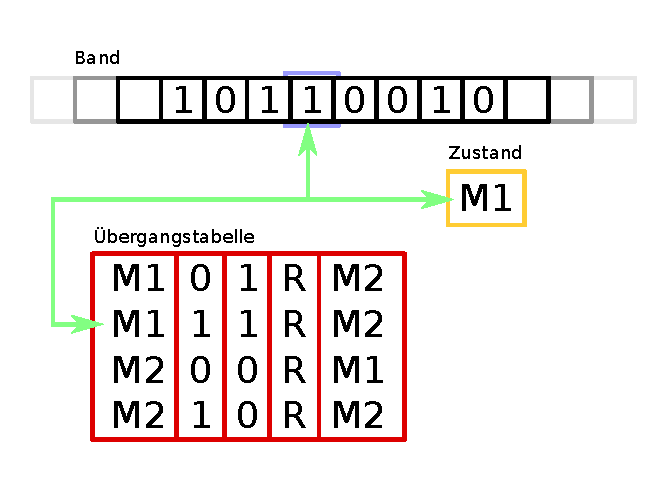
\includegraphics{img/turingmachine_visualization.pdf}
  \caption{Die Funktionsweise einer Turingmaschine visualisiert}
  \label{fig:tm_vis}
 \end{center}
\end{figure}
%
In Abbildung~\ref{fig:tm_vis} ist der Aufbau einer Turingmaschine visualisiert. Die Turingmaschine besitzt ein unendlich langes \emph{Band} (schwarz) auf welchem Zeichen aus dem Alphabet $\Gamma$ stehen. Der \emph{Cursor} (blau) befindet sich an einer bestimmten Stelle auf diesem Band und liest und schreibt Zeichen. Basierend auf der Information in welchem \emph{Zustand} (orange) sich die Turingmaschine befindet und welches \emph{Zeichen gelesen} wurde, wird eine Zeile in der \emph{Übergangstabelle} (rot) ausgewählt, die dann den Zustandübergang definiert.

Die Turingmaschine besitzt eine initiale Konfiguration. Als Konfiguration bezeichnet man das Tupel (Zustand, Band, Cursor). Die abgebildeten Turingmaschine befindet sich in einem Zustand M1, auf dem Band befinden sich die Zeichen 10110010 (aus dem Alphabet $\Sigma$) und der Cursor ist links der Mitte positioniert. Dies sei unsere initiale Konfiguration. Die weiteren Konfigurationen lassen sich durch schrittweise Ausführung der Instruktionen ableiten. \\
Aufgrund der Konfiguration können wir jetzt in der Übergangstabelle nachschlagen, welche Instruktion ausgeführt werden soll. Eine Zeile der Spalte besteht dabei aus 5 Werten: Ausgangszustand, gelesenes Zeichen, geschriebenes Zeichen, Bewegung und nächster Zustand. Dies bedeutet in Zeile~2 stimmt die Konfiguration mit den Werten überein: Wir befinden uns im Zustand M1 (ja, in diesem befinden wir uns gerade) und lesen das Zeichen ,,1`` (ja, wurde vom Cursor gelesen). Dementsprechend ist eine ,,1`` an diese Position am Band zu schreiben, nach rechts (,,R``) zu fahren und in den Zustand ,,M2`` zu wechseln. Wenn wir den nachfolgenden Schritt beobachten, wird die Zeile 3 ausgeführt: Im Zustand ,,M2`` wurde das Zeichen ,,0`` gelesen, wird das Zeichen ,,0`` geschrieben, der Cursor nach rechts (,,R``) bewegt und in den Zustand ,,M1`` gewechselt.

Erreicht die Turingmaschine einen der definierten Endzustände, wird die Eingabe als ,,akzeptiert`` (Ja) interpretiert. Kommt die Turingmaschine in einen undefinierten Zustand, wird die Eingabe ,,abgelehnt`` (Nein).

Durch das Wechseln von Zuständen und das Speichern von Zeichen auf dem Band können Daten verarbeitet werden. Der Input und Output eines ablaufenden Algorithmus' bildet die Initial- und Endkonfiguration der Turingmaschine. Die Logik bzw. das Programm ist in der Übergangstabelle kodiert. Es ist im Allgemeinen nicht möglich aus der Problembeschreibung den entsprechenden Algorithmus zu generieren, der das Problem entscheidet. Dies begründet das Tätigkeitsfeld eines Programmierers und erfordert seine menschliche Kreativität.

Eine Turingmaschine, die eine Bewegung ,,Stop`` unterstützt ist gleich mächtig wie eine Turingmaschine, die es nicht unterstützt. Hierfür muss die Anzahl der Zustände (in denen ein Stop gebraucht wird) verdoppelt werden. In den folgenden Programmen verwenden wir die Bewegung ,,Stop``.

\section{Algorithmenbeispiele auf der Turingmaschine}
%
Im Folgenden werden 3 Algorithmen für 3 verschiedene Probleme vorgestellt, die wir auf einer Turingmaschine entscheiden werden. Sie folgen jeweils unterschiedlichen Ideen und sollen dem Leser mögliche Lösungsansätze für andere äquivalente Probleme illustrieren.

\subsection{Algorithmus: Gerade oder ungerade Anzahl}
\index{Gerade oder ungerade Anzahl (Algorithmus)}
%
Gegeben sei eine Turingmaschine. Auf dem Band befindet sich eine beliebige Sequenz von Nullen (0) und Einsen (1). Der Cursor befindet sich auf der linkesten Ziffer. Gehe in den Endzustand ,,Even`` wenn sich eine gerade Anzahl an Ziffern auf dem Band befinden. Gehe in den Endzustand ,,Odd`` wenn sich eine ungerade Anzahl an Ziffern auf dem Band befinden. Die Position des Cursors in den Endzuständen ist nicht spezifiziert. Das Band muss im Endzustand gleich wie am Anfang aussehen. Schreibe das Programm der Turingmaschine, um dieses Problem zu entscheiden.

\textbf{Lösung (Tabelle~\ref{tab:odd_even}).} Der Lösungsansatz beruht darauf zwischen den zwei Zuständen ,,Even`` und ,,Odd`` zu alternieren, wobei der entsprechende Zustand repräsentiert, ob eine gerade oder ungerade Anzahl von Zeichen bisher gelesen wurde. Zu beachten ist weiters, dass die Sequenz auch die Länge $0$ umfasst und daher der Fall abgedeckt werden muss, falls sich kein Zeichen (bzw. das Blanksymbol) unter dem Startzustand befindet.
%
\begin{table}
 \begin{center}
  \begin{tabular}{ccccc}
   \hline
    Zustand & Lesen     & Schreiben & Bewegung & neuer Zustand \\
   \hline \hline
    Start   & $\square$ & $\square$ & Stop     & Even \\
    Start   & 0         & 0         & Rechts   & Odd \\
    Start   & 1         & 1         & Rechts   & Odd \\
    Even    & $\square$ & $\square$ & Stop     & Even \\
    Even    & 0         & 0         & Rechts   & Odd \\
    Even    & 1         & 1         & Rechts   & Odd \\
    Odd     & $\square$ & $\square$ & Stop     & Odd \\
    Odd     & 0         & 0         & Rechts   & Even \\
    Odd     & 1         & 1         & Rechts   & Even \\
   \hline
  \end{tabular}
  \caption{Eine Übergangstabelle für ,,Gerade oder ungerade Anzahl``}
  \label{tab:odd_even}
 \end{center}
\end{table}

\subsection{Algorithmus: 1en zählen}
\index{Einsen zählen (Algorithmus)}
%
Gegeben sei eine Turingmaschine. Auf dem Band befindet sich eine beliebige Sequenz von Nullen und Einsen (der Mindestlänge 1). Der Cursor befindet sich auf der linkesten Ziffer. Gesucht ist ein Algorithmus, welcher das Band mit Blanksymbolen überschreibt und genau so viele Einsen nebeneinander angeordnet schreiben soll, wie im String anfangs enthalten waren. Als Beispiel soll der Eingabestring ,,00101101`` zur Ausgabe ,,1111`` führen. Als weiteres Beispiel soll ,,10`` zu ,,1`` führen. Im Endzustand ,,End`` soll der Cursor auf der rechtesten 1 stehen.

\textbf{Lösung (Tabelle~\ref{tab:count_ones}).} Der Algorithmus folgt diesem Ablauf:
\begin{enumerate}
  \item Markiere Anfang (\^{}) und Ende (\$) mit zwei Hilfssymbolen
        (diese Markung wird in den Zuständen Start und Mark vorgenommen).
  \item Im Zustand \textit{Find} gehe nach rechts und suche die nächste 1.
        Ersetze sie mit einer 0 und gehe in Zustand \textit{Found} oder falls du keine 1 findest,
        finalisiere das Band.
  \item In den Zuständen \textit{Found}, \textit{Write} und \textit{Return} wird das Symbol
        auf der rechten Seite des Hilfssymbols \$ hinzugefügt und es wird zurück zur linken Seite gegangen.
  \item Beim Finalisieren lösche die Hilfssymbole \^{} und \$ und die Anfangssequenz von Nullen und Einsen
        vom Band. Gehe an die rechteste Position des Ergebnisses.
\end{enumerate}
%
\begin{table}
 \begin{center}
  \begin{tabular}{ccccc}
   \hline
    Zustand & Lesen     & Schreiben & Bewegung & neuer Zustand \\
   \hline \hline
    Start   & $\square$ & \$        & Links    & Mark \\
    Start   & 0         & 0         & Rechts   & Start \\
    Start   & 1         & 1         & Rechts   & Start \\
    Mark    & $\square$ & \^{}      & Rechts   & Find \\
    Mark    & 0         & 0         & Links    & Mark \\
    Mark    & 1         & 1         & Links    & Mark \\
    Find    & 0         & 0         & Rechts   & Find \\
    Find    & 1         & 0         & Rechts   & Found \\
    Find    & \$        & \$        & Links    & Finalize \\
    Found   & 0         & 0         & Rechts   & Found \\
    Found   & 1         & 1         & Rechts   & Found \\
    Found   & \$        & \$        & Rechts   & Write \\
    Write   & $\square$ & 1         & Links    & Return \\
    Write   & 1         & 1         & Rechts   & Write \\
    Return  & 0         & 0         & Links    & Return \\
    Return  & 1         & 1         & Links    & Return \\
    Return  & \$        & \$        & Links    & Return \\
    Return  & \^{}      & \^{}      & Rechts   & Find \\
    Finalize& 0         & 0         & Links    & Finalize \\
    Finalize& 1         & 1         & Links    & Finalize \\
    Finalize& \^{}      & $\square$ & Rechts   & Delete \\
    Delete  & 0         & $\square$ & Rechts   & Delete \\
    Delete  & 1         & $\square$ & Rechts   & Delete \\
    Delete  & \$        & $\square$ & Rechts   & Result \\
    Result  & $\square$ & $\square$ & Stop     & End \\
    Result  & 1         & 1         & Rechts   & Result \\
   \hline
  \end{tabular}
  \caption{Eine Zustandstabelle für ,,Einsen zählen``}
  \label{tab:count_ones}
 \end{center}
\end{table}

\subsection{Algorithmus: Minimum von 3 2-bit Zahlen}
\index{Minimum von 2-bit Zahlen (Algorithmus)}
%
Gegeben sei eine Turingmaschine. Auf dem Band befinden sich 6 Nullen oder Einsen. Diese sind als 3 2-bit Zahlen zu interpretieren. Schreibe rechts von diesen Zahlen jenen Wert, der das Minimum der 3 Zahlen repräsentiert und lasse das restliche Band im Anfangszustand. Der Startzustand sei ,,Start`` und der Endzustand sei ,,End``. Die initiale Cursorposition sei die linkeste Ziffer. Im Endzustand soll der Cursor ganz rechts sein.

\textbf{Lösung (Tabelle~\ref{tab:min_3bit}).} Unser Lösungsansatz beruht auf der Idee, dass wir sämtliche relevanten Informationen des Inputs in den Zuständen speichern. Wir modifizieren das Band nicht (d.h. gelesene und geschriebene Zeichen sind stets ident außer wir schreiben das Ergebnis) und die Bewegung geht stets nach rechts (außer wir terminieren). Wir lesen Ziffer für Ziffer ein und wechseln in einen entsprechenden Zustand. So wird etwa in dem Startzustand bei einem gelesenen $1$ in den Zustand $001$ gewechselt, um uns zu merken dass das kleinste Minimum $00$ war (wir haben bisher noch keine Zahl gelesen und daher wird die niedrigste Zahl $00$ verwendet) und mit der zusätzlichen $1$ merken wir uns das letzte gelesene Symbol. Dies ist bei allen Zuständen, die aus 3 Ziffern bestehen gleichartig. Wir müssen dabei in jenen Zustand wechseln, welcher das Maximum der zwei Zustände repräsentiert, die wir durch den aktuellen Zustand und das gelesene Zeichen kodiert haben. Haben wir eine gerade Anzahl an Zeichen gelesen, befinden wir uns in einem Zustand aus 2 Ziffern und sonst in einem Zustand aus 3 Ziffern. Kommen wir auf ein Blanksymbol, schreiben wir jene Zahl, die wir als Minimum im Namen des Zustands gespeichert haben.
%
\begin{table}
 \begin{center}
  \begin{tabular}{ccccc}
   \hline
    Zustand & Lesen     & Schreiben & Bewegung & neuer Zustand \\
   \hline \hline
    Start   & 0         & 0         & Rechts   & 000 \\
    Start   & 1         & 1         & Rechts   & 001 \\
    000     & 0         & 0         & Rechts   & 00 \\
    000     & 1         & 1         & Rechts   & 01 \\
    001     & 0         & 0         & Rechts   & 10 \\
    001     & 1         & 1         & Rechts   & 11 \\
    010     & 0         & 0         & Rechts   & 01 \\
    010     & 1         & 1         & Rechts   & 01 \\
    011     & 0         & 0         & Rechts   & 10 \\
    011     & 1         & 1         & Rechts   & 11 \\
    100     & 0         & 0         & Rechts   & 10 \\
    100     & 1         & 1         & Rechts   & 10 \\
    101     & 0         & 0         & Rechts   & 10 \\
    101     & 1         & 1         & Rechts   & 11 \\
    110     & 0         & 0         & Rechts   & 11 \\
    110     & 1         & 1         & Rechts   & 11 \\
    111     & 0         & 0         & Rechts   & 11 \\
    111     & 1         & 1         & Rechts   & 11 \\
    00      & $\square$ & 0         & Rechts   & 0 \\
    00      & 0         & 0         & Rechts   & 000 \\
    00      & 1         & 0         & Rechts   & 001 \\
    01      & $\square$ & 0         & Rechts   & 0 \\
    01      & 0         & 0         & Rechts   & 010 \\
    01      & 1         & 1         & Rechts   & 011 \\
    10      & $\square$ & 1         & Rechts   & 0 \\
    10      & 0         & 0         & Rechts   & 100 \\
    10      & 1         & 1         & Rechts   & 101 \\
    11      & $\square$ & 1         & Rechts   & 1 \\
    11      & 0         & 0         & Rechts   & 110 \\
    11      & 1         & 1         & Rechts   & 111 \\
    0       & $\square$ & 0         & Stop     & End \\
    1       & $\square$ & 1         & Stop     & End \\
   \hline
  \end{tabular}
  \caption{Eine Zustandstabelle für ,,Minimum von 3 2-bit Zahlen``}
  \label{tab:min_3bit}
 \end{center}
\end{table}

\section{Theoretische Erkenntnisse}
\subsection{Universelle Turingmaschine}
\index{Universelle Turingmaschine}
%
Unter einer \emph{universellen Turingmaschine} versteht man eine Turingmaschine, welche als Parameter\footnote{Unter Parameter im Kontext einer Turingmaschine versteht man einen Wert, welcher bereits auf das Band kodiert wurde, bevor die Turingmaschine gestartet wurde.} eine andere Turingmaschine entgegen nimmt und nachfolgend die einzelnen Schritte der Turingmaschine berechnet. Dabei befinden sich alle Informationen wie der aktuelle Zustand, das Band und das Programm auf dem Band der universellen Turingmaschine. Wird ein Befehl der simulierten Turingmaschine ausgeführt, wird am Band nach der entsprechenden Instruktion nachgeschlagen und der Befehl ausgeführt.

Die genaue Implementierung wird hier nicht weiter präzisiert, da es sich nur um Überlegungen hinsichtlich Kodierungen handelt.
%
\subsection{Mehrbandturingmaschinen}
\index{Mehrbandturingmaschine}
%
Eine Erweiterung der Turingmaschine besteht darin mehr als 1 Band zu verwenden. Dies hilft insbesondere bei der Organisation der Daten bei der Implementierung von Algorithmen. Betrachten wir etwa ein Graphenproblem, hilft es beispielweise auf einem Band den aktuell betrachteten Knoten zu speichern und auf den weiteren Bändern zwei anliegende Kanten. In dem Fall müssen wir die Wanderungen nicht ausformulieren, wenn wir die Bänderdaten von einem anderen Band lesen wollen und diese Bänder nebeneinander angeordnet werden.

Jede Mehrbandturingmaschine kann durch eine Turingmaschine mit 1 Band simuliert werden.

Die Frage, die sich jedoch stellt, ist: Hat diese Erweiterung Auswirkungen auf die Komplexität der Probleme? Wie es sich herausstellt, handelt es sich nur um einen polynomiallen Mehraufwand.
%
\subsection{Nicht-Determinismus}
\label{sec:nondeterminism}
\index{Nicht-Determinismus}
\index{Orakel (Turingmaschine)}
%
Der Nichtdeterminismus ist ein wichtiges Konzept für die theoretische Informatik. Grundsätzlich handelt es sich bei der Übergangsfunktion der Turingmaschine um eine Abbildung des gelesenen Zeichens und des aktuellen Zustands auf den neuen Zustand, das zu schreibende Zeichen und eine Bewegung. Nichtdeterminismus beschreibt den Zustand eines Systems in dem der Übergang von einem Zustand der Maschine in den nächsten Zustand nicht wohldefiniert und eindeutig ist. In anderen Worten auch: Für eine gegebene Konfiguration der Turingmaschine gibt es mehrere Möglichkeiten in den nächsten Zustand zu kommen.

Im Kontext der Komplexitätstheorie spricht man bei Nichtdeterminismus von den sogenannten \emph{Orakelturingmaschinen}. Liegen mehrere Zustandübergänge für eine Konfiguration vor, befragt die Turingmaschine die (zur Verfügung stehende) Orakelturingmaschine. Diese antwortet stets mit jenem Übergang, welcher direkt zur richtigen Lösung führt. Diese Hervorsagefähigkeit begründet ihren Namen ,,Orakel``.
%
\subsection{Unentscheidbarkeit des Halteproblems}
\index{Halteproblem}
%
\index{Turing-berechenbar}
Alan Turing konnte 1936~\cite{Turing01011937} überraschenderweise beweisen, dass es einfache, nur mit ja oder nein beantwortbare Fragestellungen (auch Entscheidungsprobleme genannt) gibt, die sich mit Turingmaschinen \emph{nicht} vollständig beantworten lassen, obwohl eine klar definierte Antwort offensichtlich existieren muss. Dabei ist es für die eigentliche Fragestellung selbstverständlich rein logisch gesehen unwichtig, \emph{wie} die Antwort herausgefunden wird, sie muss nur der Wahrheit entsprechen und liegt sozusagen unmittelbar vor, während eine Turingmaschine die korrekte Antwort erst Schritt-für-Schritt \emph{berechnen} muss.

Turing bewies nun, dass es keine Turingmaschine $\mathbf{H}$ geben \emph{kann}, die in jedem Fall nach endlich vielen Schritten die richtige Antwort auf die Fragestellung liefert, ob eine beliebige andere Turingmaschine $\mathbf{M}$ bei anfänglichen Bandinhalt $\mathbf{I_M}$ irgendwann anhält oder stattdessen für immer weiterrechnet (das sogenannte \href{http://de.wikipedia.org/wiki/Halteproblem}{Halteproblem}).

Unter Annahme der \href{http://de.wikipedia.org/wiki/Church-Turing-These}{Church-Turing These} lassen sich solche Fragestellungen daher mittels bekannter Methoden nicht eindeutig entscheiden, und man bezeichnet sie entsprechend als \emph{unentscheidbar} (ohne Annahme der Church-Turing These kann man nur sagen, dass das Halteproblem nicht \emph{Turing-berechenbar} ist, allerdings ist die Church-Turing These allgemein akzeptiert).

Der Beweis der Unentscheidbarkeit des Halteproblems folgt durch einen Widerspruch, welcher nur beseitigt werden kann, wenn folgende Annahme zurückgenommen wird (d.h.\ die Turingmaschine $\mathbf{H}$ kann es nicht geben).

\paragraph{Annahme:} Es gibt eine Turingmaschine $\mathbf{H}$, die für eine beliebige Turingmaschine $\mathbf{M}$ und einen beliebigen Input $\mathbf{I_M}$ in endlich vielen Schritten herausfindet, ob $\mathbf{M}$ mit anfänglichen Bandinhalt $\mathbf{I_M}$ irgendwann anhält oder nicht. Die Turingmaschine $\mathbf{H}$ schreibt als Antwort aufs Band \emph{ja}, falls $\mathbf{M}$ mit $\mathbf{I_M}$ irgendwann anhält, und \emph{nein}, falls $\mathbf{M}$ mit Input $\mathbf{I_M}$ nicht anhält, und bleibt sofort danach stehen (siehe Abbildung~\ref{fig:haltingproblem1}).

\begin{figure}[h]
\begin{minipage}[h]{0.475\textwidth}
\centering
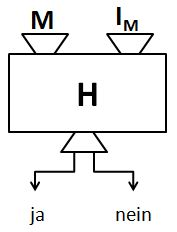
\includegraphics[width=3cm]{img/haltingproblem1.jpg}
    \caption{Turingmaschine $\mathbf{H}$.}
    \label{fig:haltingproblem1}
\end{minipage}
%
\begin{minipage}[h]{0.475\textwidth}
\centering
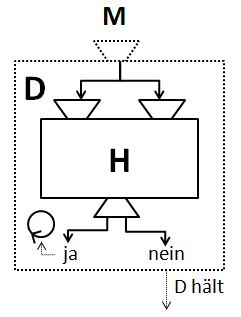
\includegraphics[width=3cm]{img/haltingproblem2.jpg}
    \caption{Turingmaschine $\mathbf{D}$.}
    \label{fig:haltingproblem2}
\end{minipage}
\end{figure}

Für den Beweis wird eine weitere Turingmaschine $\mathbf{D}$ (siehe Erklärung weiter unten, warum hier der Buchstabe \emph{D} verwendet wird) definiert, die sich wie folgt verhält (siehe Abbildung~\ref{fig:haltingproblem2}):
\begin{itemize}
  \item Bei Eingabe von (der kodierten Form von) $\mathbf{M}$ simuliert $\mathbf{D}$  die Turingmaschine $\mathbf{H}$ mit Eingabe $\mathbf{I_M = M}$.
  \item $\mathbf{H}$ antwortet hier also mit \emph{ja} oder \emph{nein}, je nachdem ob $\mathbf{M}$ bei Verwendung des eigenen kodierten Programmcodes (also von $\mathbf{M}$) als Input anhält oder nicht.
  \item Sobald die Simulation von $\mathbf{H}$ fertig ist (was nach endlich vielen Schritten sicher passiert, so die Annahme), so verhält sich $\mathbf{D}$ zusätzlich noch wie folgt:
    \begin{itemize}
      \item Falls $\mathbf{H}$ als Resultat \emph{ja} ausgegeben hat, geht $\mathbf{D}$ in eine Endlosschleife.
      \item Falls $\mathbf{H}$ als Resultat \emph{nein} ausgegeben hat, hält $\mathbf{D}$  an.
    \end{itemize}
\end{itemize}

\noindent Nun wird der kodierte Programmcode von $\mathbf{D}$ in die Turingmaschine $\mathbf{D}$ als Input eingegeben, d.h.\ $\mathbf{D}$ wird mit Programminput $\mathbf{D}$ ausgeführt. Es gibt dann nur folgende zwei Fälle:

\begin{itemize}
  \item Falls $\mathbf{D}$ mit der Eingabe der kodierten Form von $\mathbf{D}$ anhielte, dann müsste die Simulation von $\mathbf{H}$, sobald diese fertig ist, also knapp \emph{vor} dem Ende der Ausführung von $\mathbf{D}$, ein \emph{nein} ausgegeben haben. Dies entspricht aber der Evaluierung des Anhaltens von $\mathbf{D}$ mit der Eingabe $\mathbf{D}$, d.h.\ $\mathbf{D}$ mit der Eingabe $\mathbf{D}$ dürfte dementsprechend \emph{nicht} angehalten haben. Da $\mathbf{D}$ mit der Eingabe $\mathbf{D}$ also sowohl halten als auch nicht halten müsste, ergibt sich in diesem Fall ein Widerspruch.
  \item Falls $\mathbf{D}$ mit der Eingabe der kodierten Form von $\mathbf{D}$ in eine Endlosschleife ginge, also \emph{nicht} anhielte, dann müsste die Simulation von $\mathbf{H}$ vor dem übergang in die Endlos\-schleife bei der Ausführung von $\mathbf{D}$ ein \emph{ja} ausgegeben haben. Letzteres entspricht aber der Evaluierung des Anhaltens von $\mathbf{D}$ mit der Eingabe $\mathbf{D}$, d.h.\ $\mathbf{D}$ mit der Eingabe $\mathbf{D}$ müsste dementsprechend angehalten haben. Da $\mathbf{D}$ mit der Eingabe $\mathbf{D}$ also sowohl nicht halten als auch halten müsste, ergibt sich auch in diesem Fall ein Widerspruch.
\end{itemize}

\noindent Beide Fälle führen also zu einem Widerspruch. Alles außer der Annahme, dass $\mathbf{H}$ existiert, ist nachvollziehbar und korrekt $\Rightarrow$ die einzige Möglichkeit, die genannten Widersprüche zu umgehen, ist die Annahme zu verwerfen.~Q.E.D.\newline

\noindent Es \emph{kann} also keine solche Turingmaschine geben, die immer entscheiden kann, ob eine beliebige andere Turingmaschine irgendwann in ihren Berechnungen anhält. über die Church-Turing-These gilt dies auch für jegliche Algorithmen (und damit für alle Arten rationaler Gedankengänge).

\paragraph{Erklärung der Bezeichnung der Turingmaschine $\mathbf{D}$ (der entsprechende Gedankengang ist eine alternative Form des Beweises):} Der Buchstabe \emph{D} steht für Diagonalisierungsargument. Und zwar betrachtet man eine Tabelle, deren Zeilen und Spalten mit allen überhaupt möglichen Kodierungen von Turingmaschinen und allen ihren möglichen Inputs für $\mathbf{H}$, je\-weils aufsteigend geordnetet, beschriftet sind. Dies geht z.B.\ mittels einer binären Kodierung, falls Programme und Inputs für $\mathbf{H}$ nur mit Nullen und Einsen beschrieben werden, also genauso wie für konventionelle heute gebräuchliche Hardware. Im Feld der Tabelle in der Zeile, deren Beschriftung $\mathbf{M}$ kodiert, und der Spalte, deren Beschriftung $\mathbf{I_M}$ kodiert, steht $\mathbf{0}$ falls die Turingmaschine $\mathbf{M}$ mit Input $\mathbf{I_M}$ anhält, und $\mathbf{1}$ falls sie nicht anhält. Dann entsprechen die Werte in der \emph{Diagonale} in der Tabelle genau dem Verhalten von $\mathbf{D}$, wenn der Wert $\mathbf{1}$ bedeutet, dass $\mathbf{D}$ \emph{anhält} (also genau \emph{umgekehrt} wie für $\mathbf{M}$!), und $\mathbf{0}$ dass sie nicht anhält. Dann entsprechen die Werte in Zeile (und Spalte) mit der Kodierung von $\mathbf{M}$ in der \emph{Diagonale} in der Tabelle genau dem Verhalten von $\mathbf{D}$ mit Input $\mathbf{M}$, wenn der Wert $\mathbf{1}$ bedeutet, dass $\mathbf{D}$ mit Input $\mathbf{M}$ \emph{anhält} (also genau \emph{umgekehrt} wie für $\mathbf{M}$!), und $\mathbf{0}$ dass sie nicht anhält.

Der Widerspruch ergibt sich bei dieser Sichtweise daraus, dass ja $\mathbf{D}$ ebenfalls eine Tu\-ringmaschine ist, die auch selbst mit der gleichen Methode wie $\mathbf{M}$ und $\mathbf{I_M}$ kodiert werden kann. Ihre Ausführung auf sich selbst als Input entspricht also ebenfalls einem Feld in der Diagonale, das dann allerdings gleichzeitig sowohl den Wert $\mathbf{0}$ als auch den Wert $\mathbf{1}$ enthalten müsste, was natürlich nicht sein kann --- dieses Feld in der Diagonale und damit auch die Kodierung von $\mathbf{D}$ sowie in weiterer Folge $\mathbf{H}$ können daher nicht existieren. Gemäß diesem Beweis ist das Halteproblem also ebenfalls unentscheidbar.~Q.E.D.

\paragraph{Das $3n+1$ Problem:} Dieses Problem, auch bekannt unter der Bezeichnung \href{http://de.wikipedia.org/wiki/Collatz-Problem}{Collatz-Problem}, zählt zu den bekanntesten ungelösten mathematischen Problemen. Sei $n$ eine natürliche Zahl. Falls $n$ gerade ist, dann fahre mit $n/2$, sonst mit $3n+1$ fort, bis durch wiederholte Anwendung dieser beiden Formeln die Zahl $1$ erreicht wird. Die Frage ist, ob der Algorithmus bei \emph{jedem} ganzahligen Anfangswert größer als $0$ die Zahl $1$ erreicht und damit anhält. Trotz größter Anstrengungen ist diese Frage bisher unbeantwortet, und für mehrere Verallgemeinerungen konnte bewiesen werden, dass sie unentscheidbar sind.

\subsection{Unentscheidbarkeit des Korrektheitsproblems}
Es gibt unzählige andere unentscheidbare Probleme\footnote{Laut dem \href{http://de.wikipedia.org/wiki/Satz_von_Rice}{Satz von Rice} ist \emph{jede} nicht-triviale Fragestellung die Turingmaschinen betrifft unentscheidbar.}, zum Beispiel das für die Informatik bedeutsame sogenannte \emph{Korrektheitsproblem}, bei dem es darum geht herauszufinden ob ein Algorithmus einer Spezifikation entspricht oder nicht. Klarerweise wäre es sehr wünschenswert, automatisch die Einhaltung einer Spezifikation überprüfen zu können. Leider lässt sich die Unentscheidbarkeit des Korrektheitsproblems leicht mittels eines sogenannten Reduktionsbeweises zeigen, wodurch sich dieser Wunsch als prinzipiell unerfüllbar erweist.

In dem Beweis wird das Halteproblem mittels einer sogenannten Reduktion (eine einfache Transformation, die problemlos ausprogrammiert werden kann) auf eine bestimmte Form des Korrektheitsproblems reduziert (dieser Begriff ergibt sich daraus, dass sich das Halteproblem dadurch sozusagen als eine vereinfachte, also eingeschränkte, sprich reduzierte Version des Korrektheitsproblems herausstellt). Wäre nun das allgemeine Korrektheitspro\-blem entscheid\-bar, würde sich aus der Reduktion ein funktionierender Algorithmus für das Halteproblem ergeben, was im Widerspruch zur bereits gezeigten Unentscheidbarkeit des Halteproblems stünde. Deshalb \emph{muss}, damit dieser Widerspruch umgangen werden kann, auch das Korrekt\-heitsproblem unentscheidbar sein.

Im Falle des Korrektheitsproblems müssen wir also bloß eine Reduktion angeben, die zu jeder beliebigen Instanz des Halteproblems eine entsprechende Instanz des Korrektheits\-problems mit gleicher ja/nein Antwort konstruiert. Sei $\mathbf{M}$ eine beliebige Turingmaschine mit einem beliebigen Input $\mathbf{I_M}$. Die Reduktion besteht nun darin, eine neue Turingmaschine $\mathbf{M'}$ zu konstruieren, indem wir übergangsregeln zu $\mathbf{M}$ so hinzuzufügen, dass nach dem Stehenbleiben des ursprünglichen Programms in mehreren zusätzlichen Schritten das gesamte Band mit Nullen überschrieben wird, schließlich eine einzelne $1$ darauf geschrieben wird und $\mathbf{M'}$ unmittelbar danach stehen bleibt. Dies ist möglich, da wir ohne Verlust der Allgemeinheit erzwingen können, dass eine Turingmaschine, hier $\mathbf{M}$, immer nur in \emph{einem} speziellen Endzustand anhalten kann.

\begin{figure}[h]
\centering
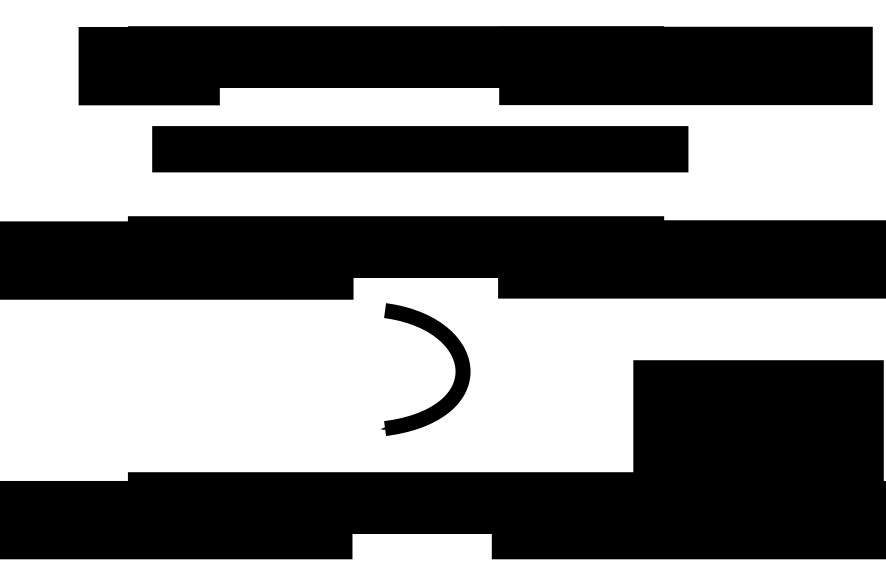
\includegraphics[width=12cm]{img/correctnessproblem}
\caption{Reduktion des Halteproblems auf das Korrektheitsproblem.}
\label{fig:correctnessproblem}
\end{figure}

Die Instanz des Korrektheitsproblem wird nun formuliert als die Frage, ob das Programm $\mathbf{M'}$ mit der gegebenen Spezifikation \glqq{}Bei Input $\mathbf{I_M}$ liefere den Wert $1$ zurück\grqq{} übereinstimmt. Klarerweise wird das \emph{genau dann und nur dann} passieren, wenn $\mathbf{M}$ mit Input $\mathbf{I_M}$ anhält.

Wenn es nun eine Turingmaschine $\mathbf{K}$ gäbe, die diese einfache Form des Korrektheitspro\-blems \emph{entscheiden} könnte (genau dies ist die zweifelhafte Annahme, die wir weiter unten wieder zurücknehmen müssen), dann würde durch obige Reduktion auch ein Algorithmus für das Halteproblem vorliegen: er würde zuerst $\mathbf{M'}$ konstruieren und dann $\mathbf{K}$ auf $\mathbf{M'}$ mit Input $\mathbf{I_M}$ loslassen, und das ja/nein Ergebnis der Berechnung von $\mathbf{K}$ als Ergebnis von $\mathbf{H}$ auswerfen (siehe Abbildung~\ref{fig:correctnessproblem}).

Dies steht allerdings im Widerspruch zur Unentscheidbarkeit des Halteproblems, demge\-mäß es ja keinen solchen Algorithmus geben kann. Daher müssen wir die oben genannte Annahme, dass eine solche Turingmaschine $\mathbf{K}$ existieren kann, zurücknehmen, und damit ist natürlich auch das allgemeine Korrektheitsproblem unentscheidbar.~Q.E.D.\newline

\noindent Für die Softwareentwicklung bedeutet dies, dass im Allgemeinen leider \emph{weder} eine automatisierte überprüfung (auch \emph{formale Verifikation} genannt) einer übereinstimmung zwischen einem Programm (bzw.\ seines source codes) und seiner Spezifikation, \emph{noch} eine händische durch einen rational vorgehenden Menschen möglich ist.
